\documentclass[a4paper,12pt]{article}

\usepackage{geometry}
\usepackage{polski}
\usepackage{amsmath}
\usepackage{ragged2e}
\usepackage{graphicx}
\usepackage{xcolor}
\usepackage{siunitx}

\graphicspath{ {./images/} }

\newcommand\crule[3][black]{\textcolor{#1}{\rule{#2}{#3}}}

\geometry{
 a4paper,
 total={170mm,257mm},
 left=20mm,
 top=20mm,
 }

\begin{document}
\title{Układy Elektroniczne - Filtry bierne i filtry aktywne}
\author{Grzegorz Litarowicz \\ Piotr Moszkowicz} 
\date{\today}
\maketitle
\pagenumbering{roman}

\newpage
\begin{justify}
\tableofcontents
\newpage
\pagenumbering{arabic}

\section{Cel i zakres ćwiczenia}

Celem ćwiczenia jest zrozumienie propagacji sygnałów zmiennych w czasie przez układy filtracji oparte na elementach rezystancyjno-pojemnościowych. Wyznaczenie doświadczalne amplitudowych charakterystyk częstotliwościowych oraz obserwacja odpowiedzi układów RC na sygnał napięciowego skoku jednostkowego. 

\section{Schemat układu pomiarowego dla filtrów biernych}

\begin{figure}[h]
\centering
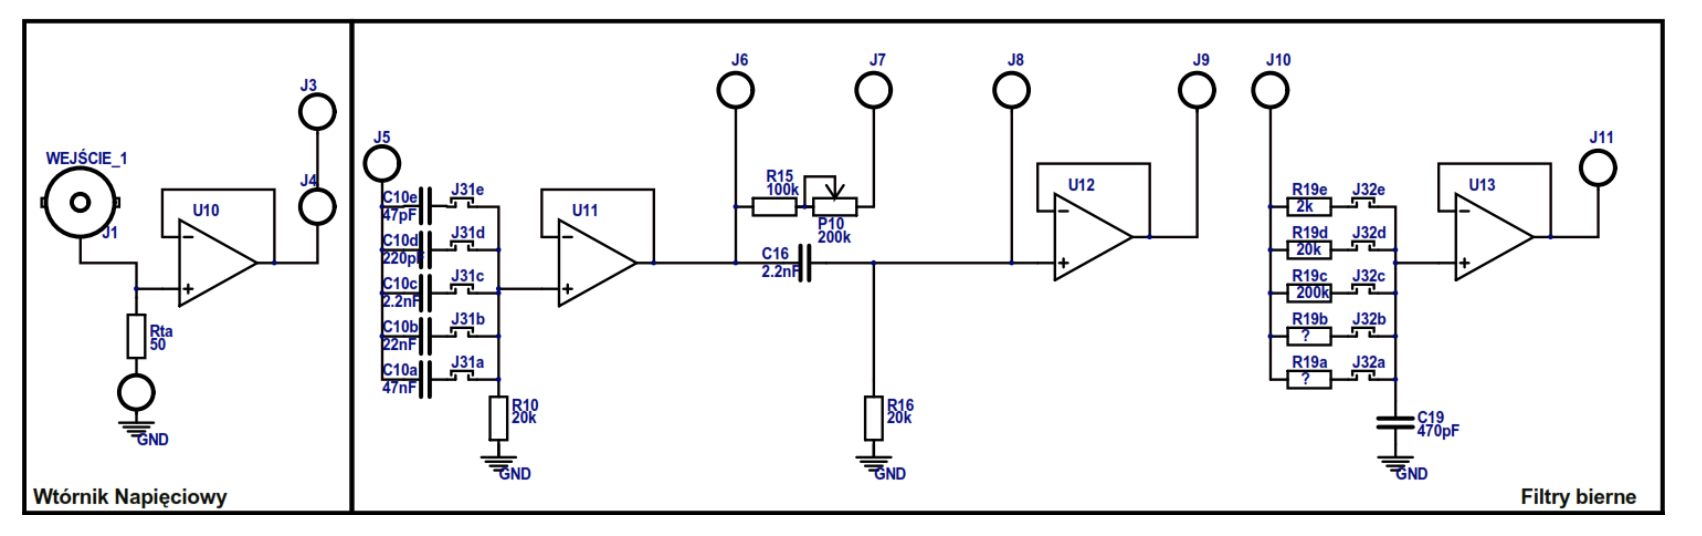
\includegraphics[width=15cm, height=5cm]{schemat_bierne}
\end{figure}

\section{Schemat układu pomiarowego dla filtrów aktywnych}

\begin{figure}[h]
\centering
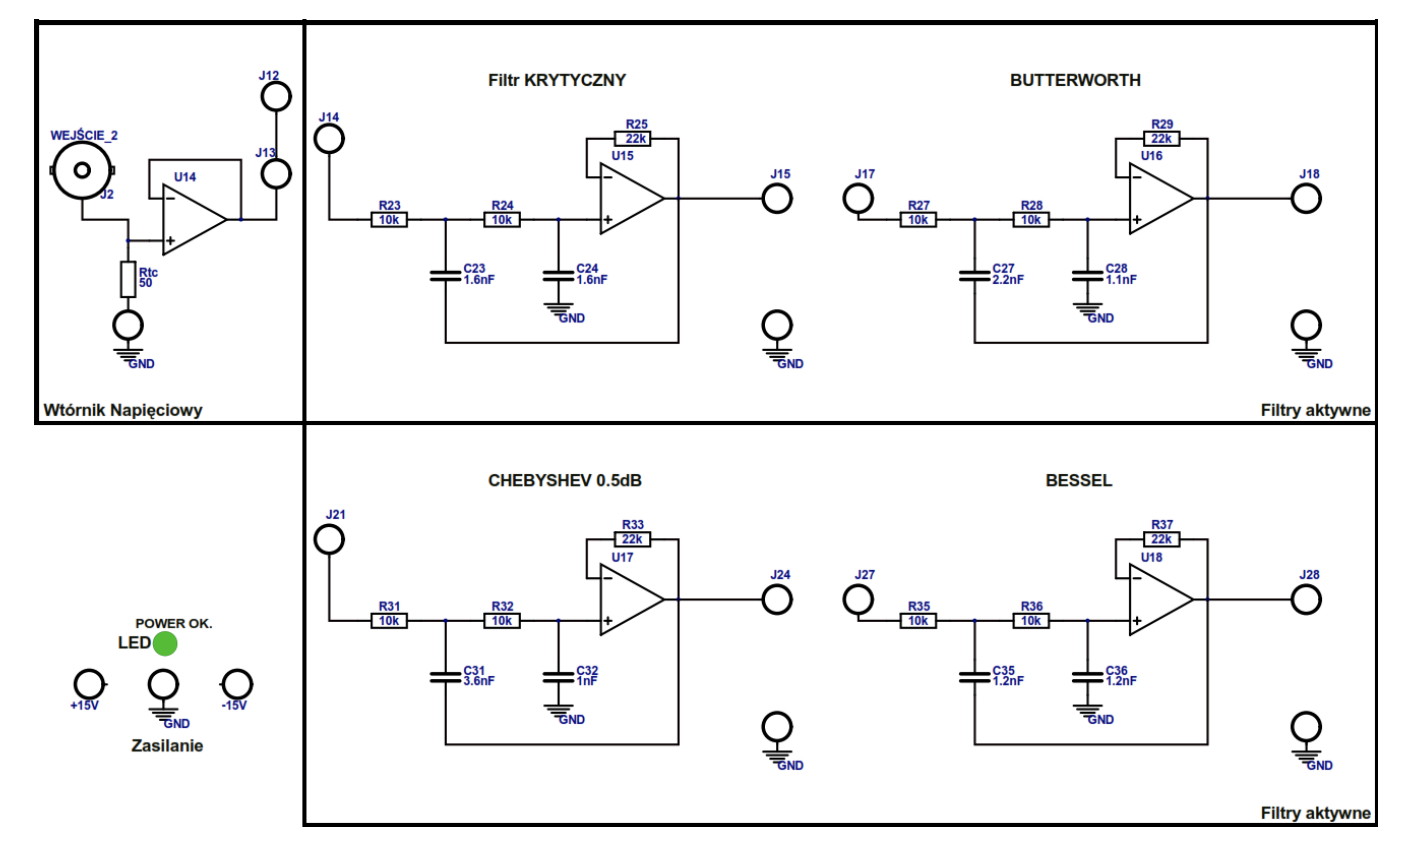
\includegraphics[width=15cm, height=9cm]{schemat_aktywne}
\end{figure}


\section{Pomiary i wyniki}

\subsection{Filtr górnoprzepustowy I rzędu}

W naszym przypadku skorzystaliśmy z kondensatora C10b o pojemności $C = 22nF$. 

\begin{figure}[h]
\centering
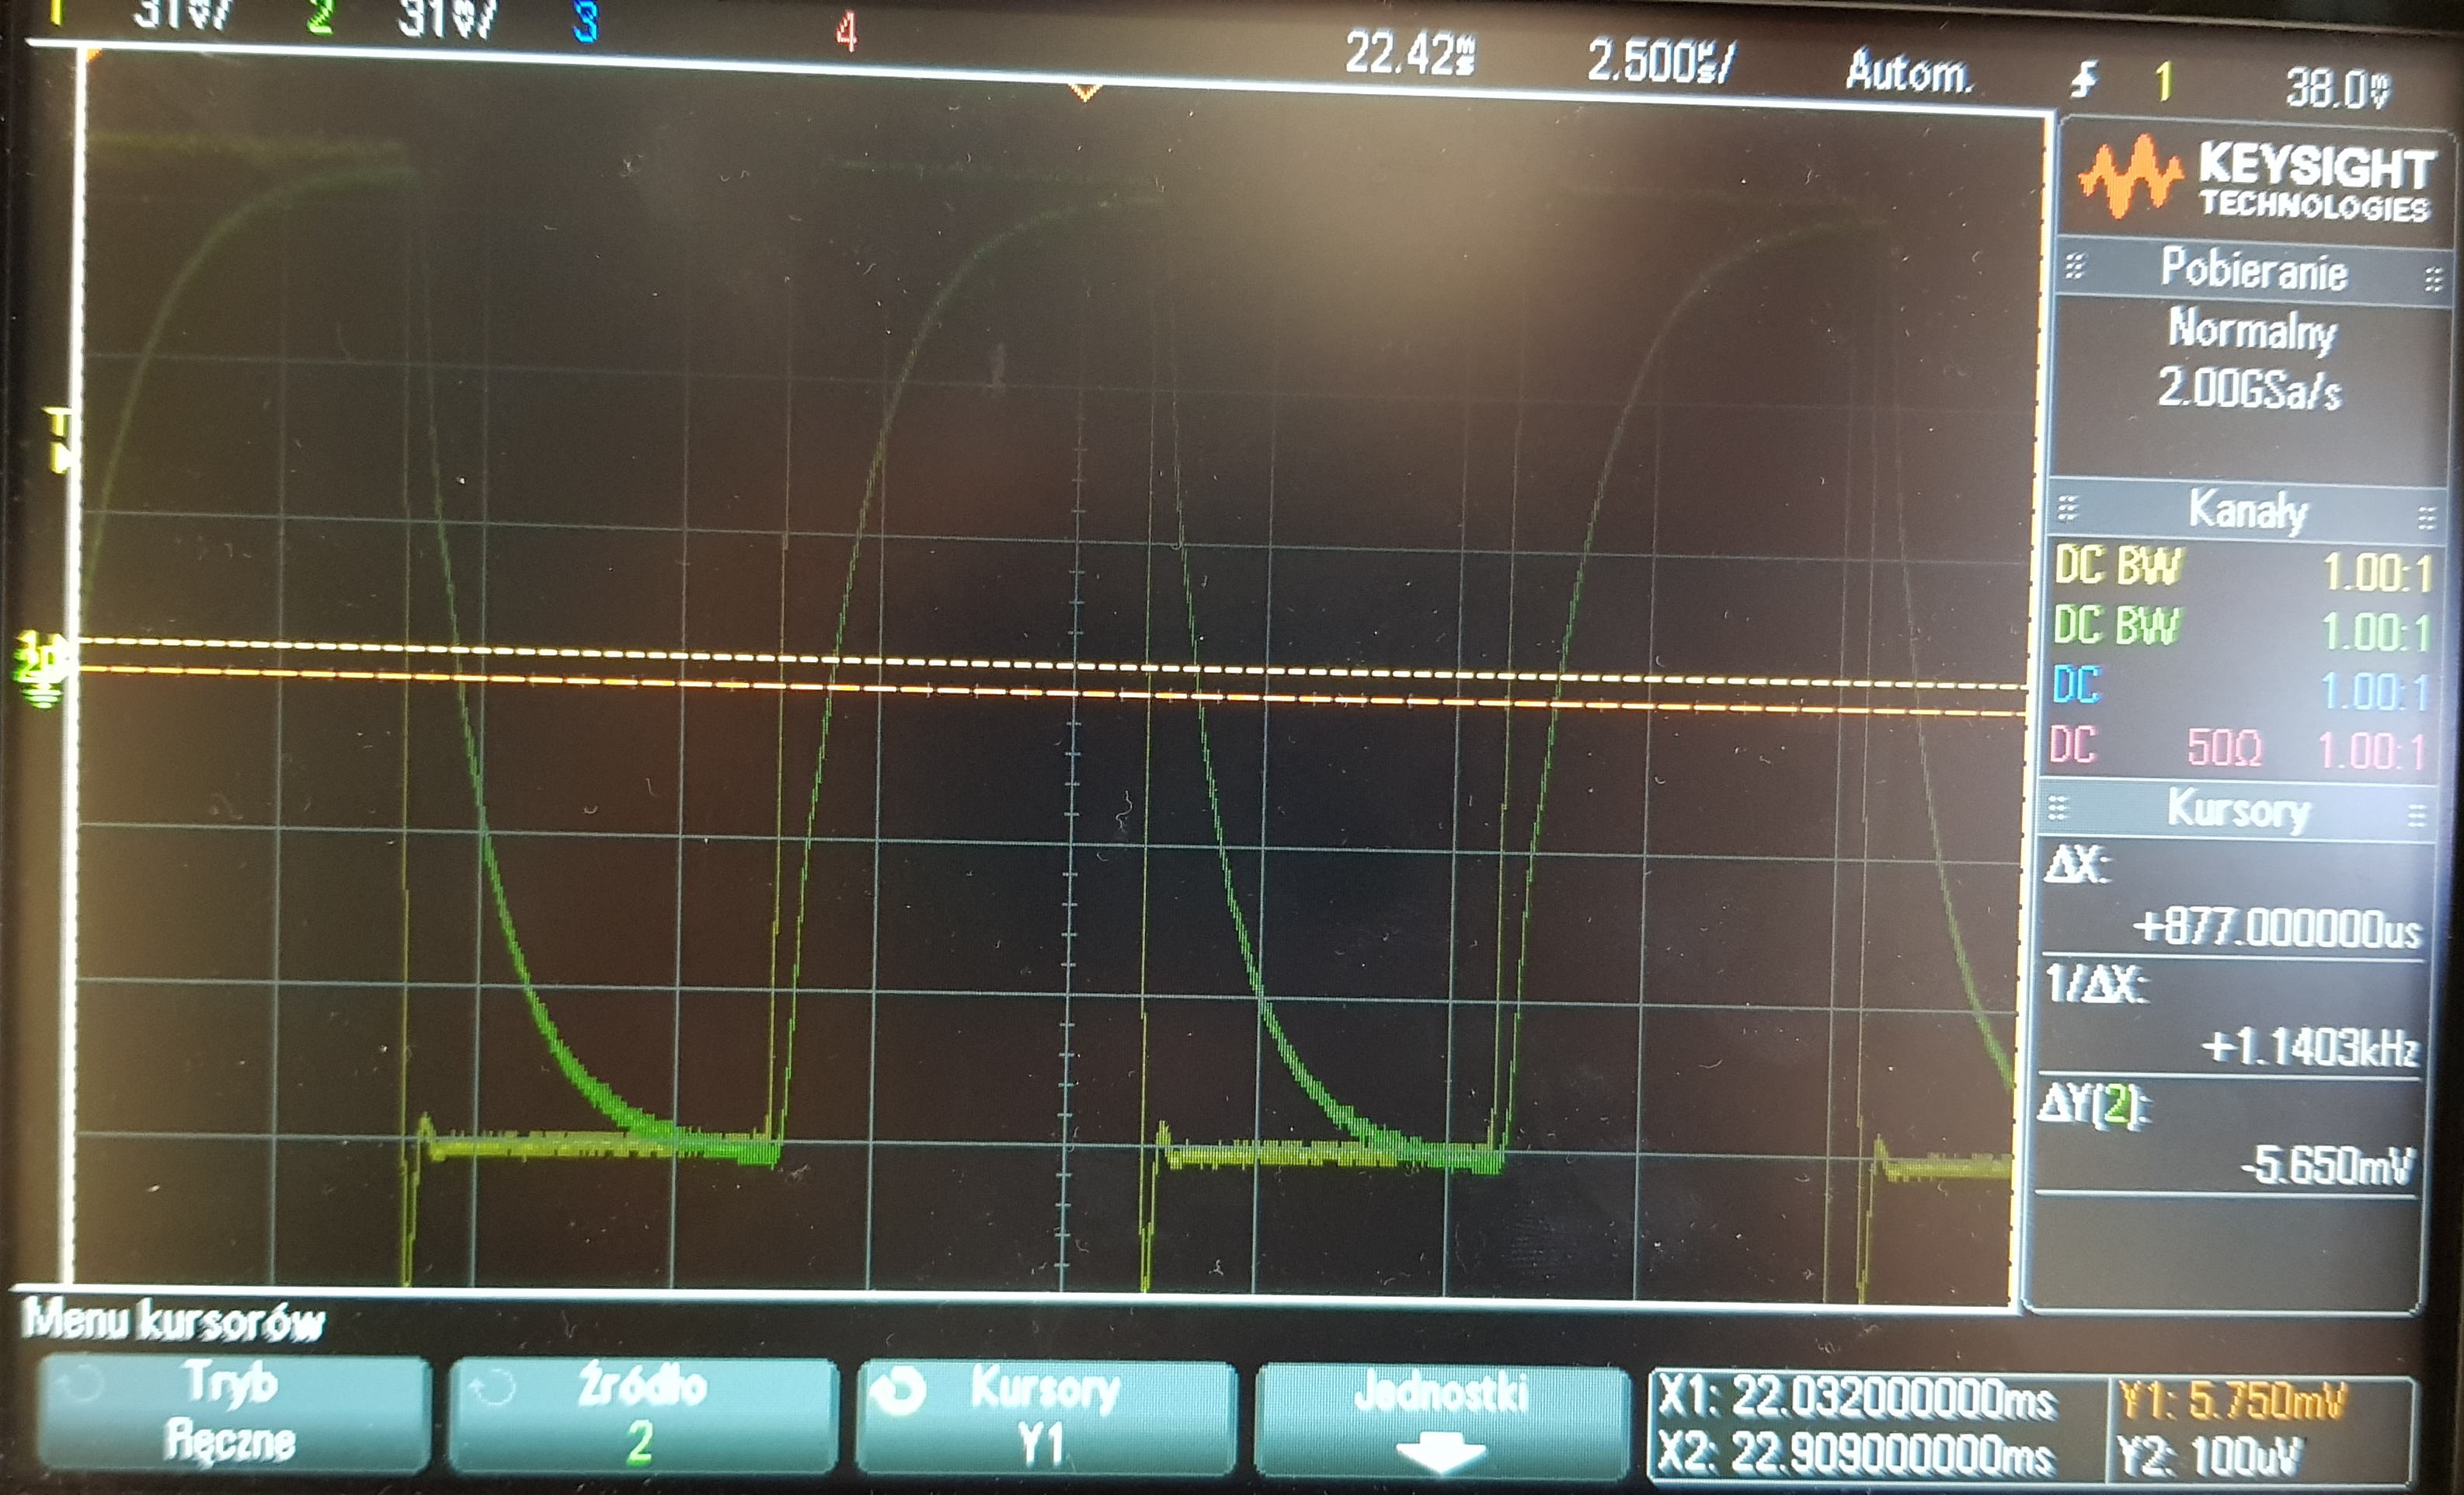
\includegraphics[width=15cm, height=9cm]{gorny_1}
\end{figure}

\begin{figure}[h]
\centering
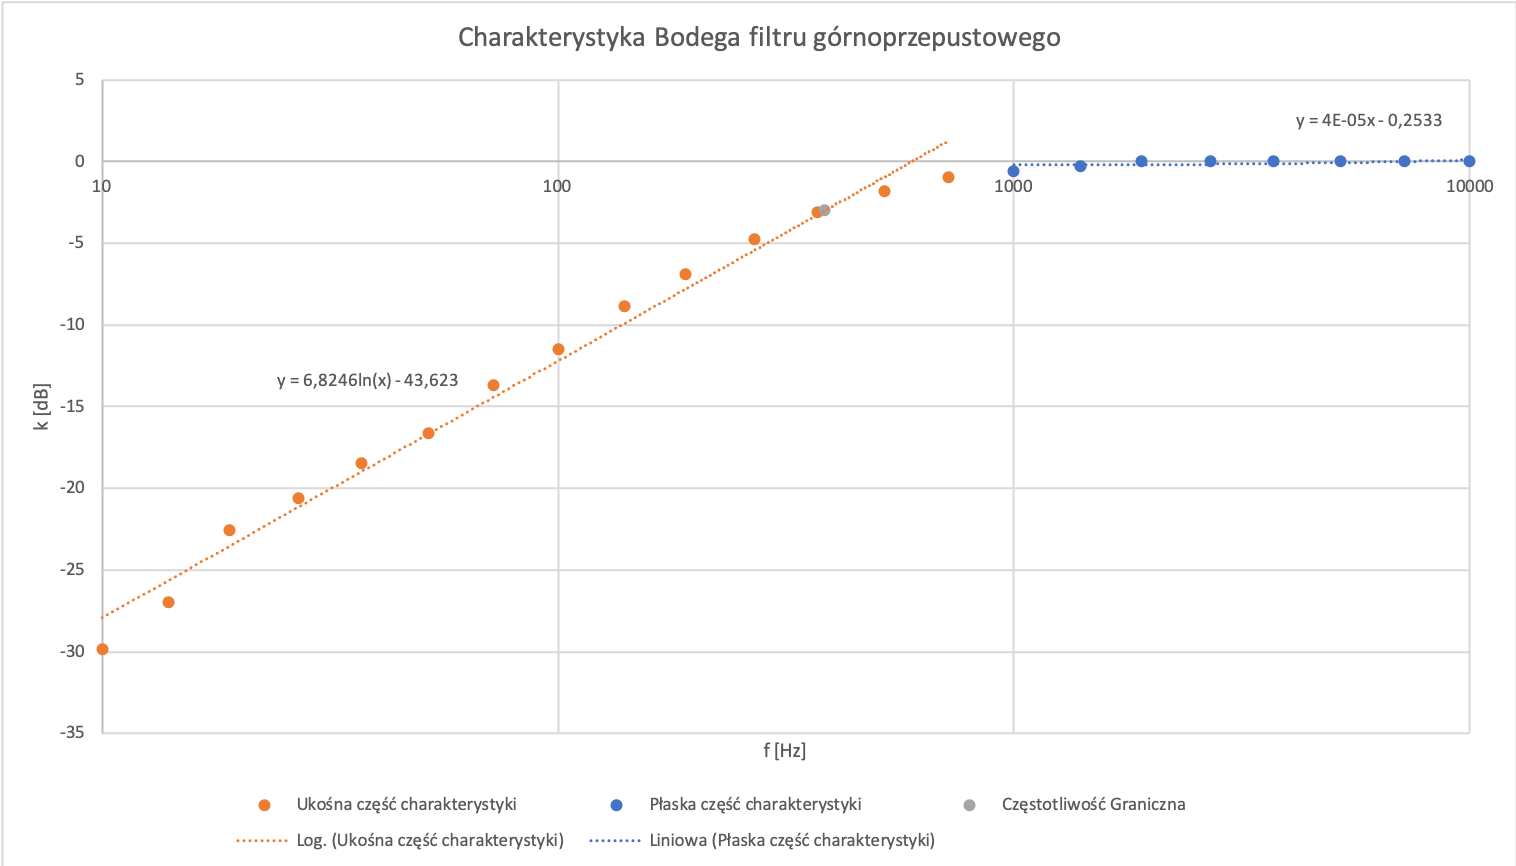
\includegraphics[width=15cm, height=9cm]{1_wykr}
\end{figure}

\paragraph{Teoretyczna częstotliwość graniczna $f_{g} = 360Hz$}
\paragraph{Zbadana częstotliwość graniczna $f_{g} = 384.98Hz$}

\paragraph{Wartość zbadana częstotliwości granicznej wyznaczyliśmy dopasowując eksponentę do wartości otrzymanych w trakcie pomiarów, a następnie po przekształceniu wzoru podstawiliśmy 3 dB. Jak widać na porównaniu wartości powyżej zbadana wartość częstotliwości trzydecybelowej jest zbliżona do wartości teoretycznej.}

\paragraph{Wartość współczynnika narastania ukośnej części charakterystyki $a = 6.8246$}
\paragraph{Wartość współczynnika narastania płaskiej części charakterystyki $a = 4e-05$}

\paragraph{Jak widać powyżej współczynnik części płaskiej jest bardzo mały, a więc filtr przepuszcza górne częstotliwości zgodnie z oczekiwaniami. }

\paragraph{Zbadane narastanie wyniosło $15.71 \frac{dB}{dek}$, ta wartość trochę odbiega od wartości teoretycznej $20 \frac{dB}{dek}$.}

\newpage

\subsection{Filtr dolnoprzepustowy I rzędu}

W naszym przypadku skorzystaliśmy z rezystora R19e o rezystancji $R = 2k \Omega$. 

\begin{figure}[h]
\centering
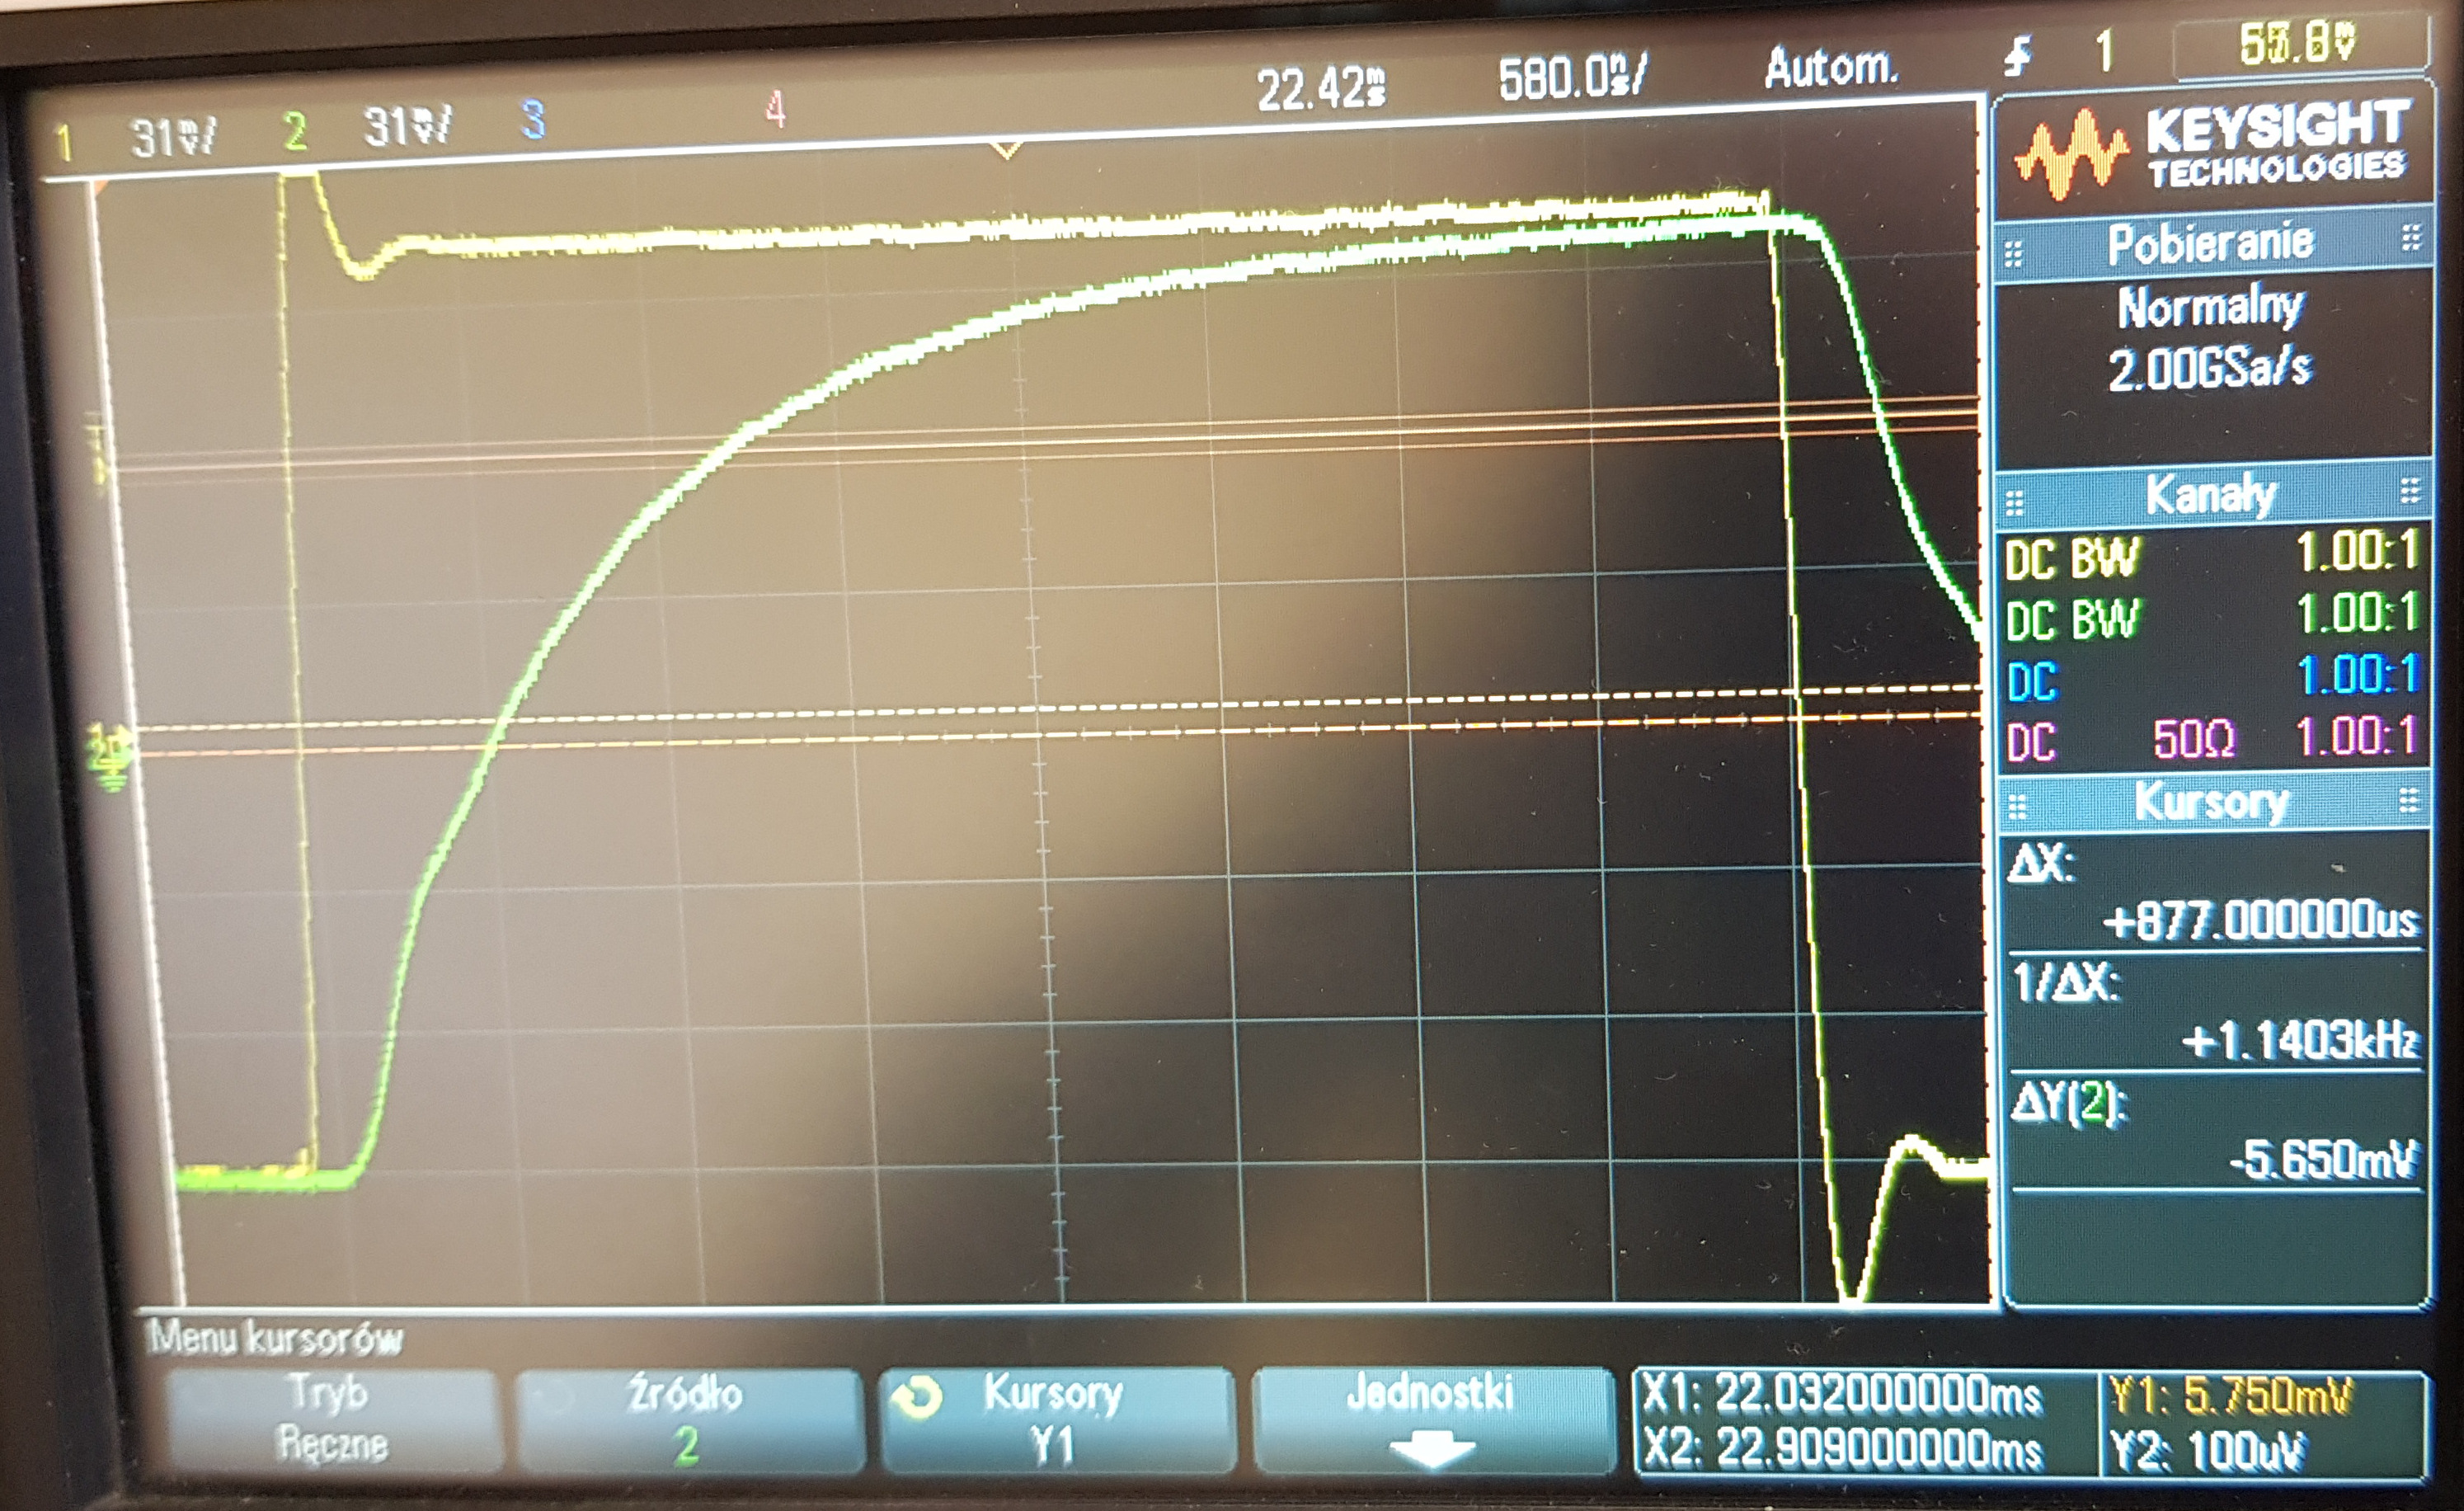
\includegraphics[width=15cm, height=9cm]{dolny_1}
\end{figure}

\begin{figure}[h]
\centering
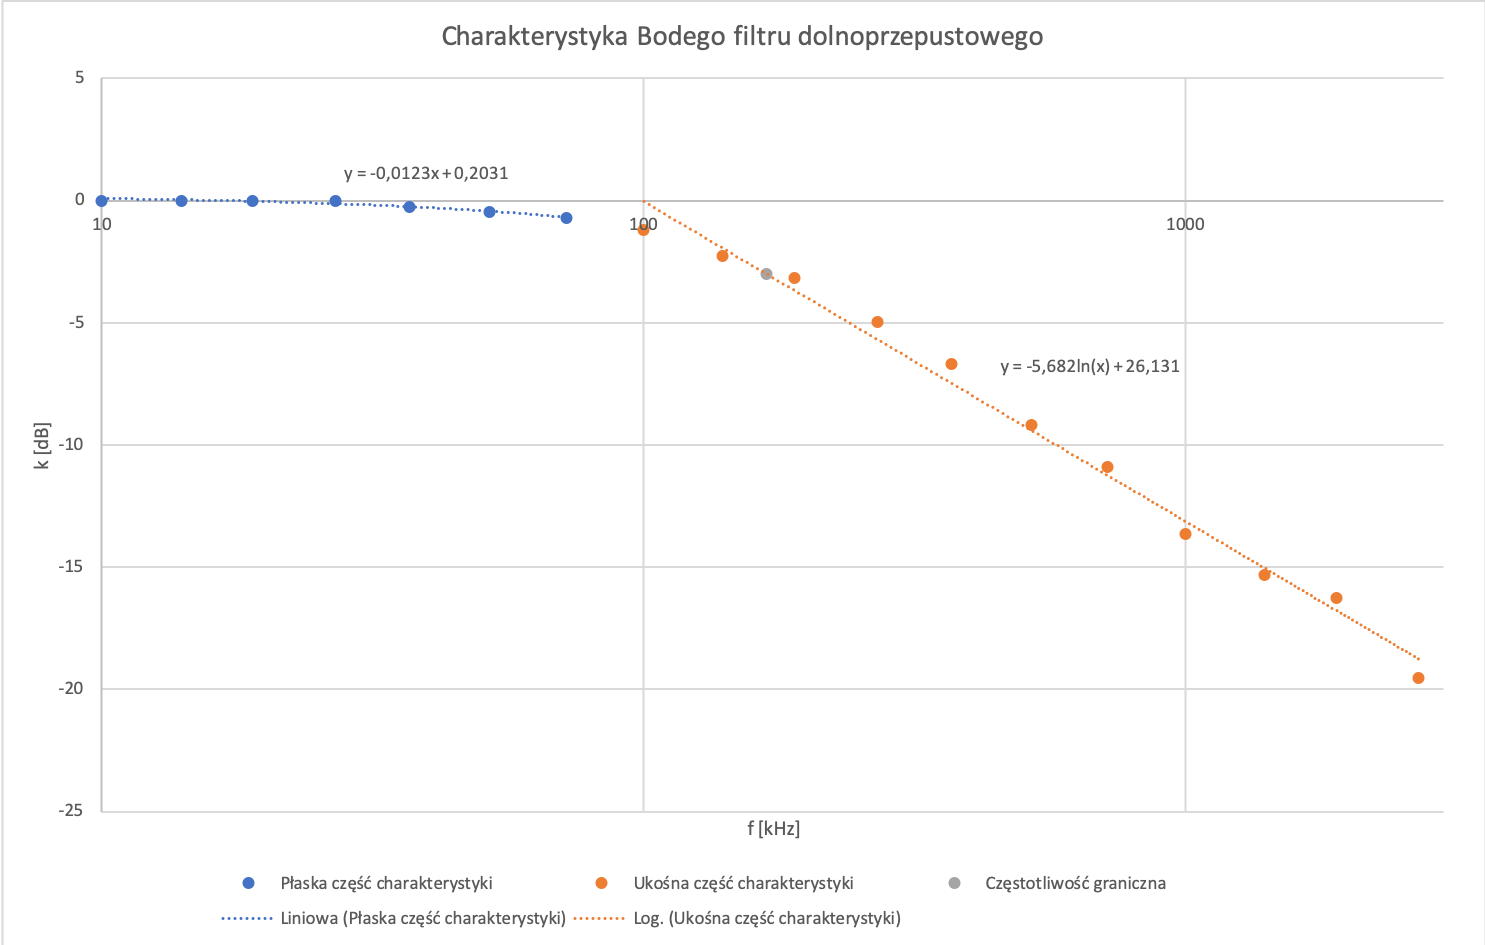
\includegraphics[width=15cm, height=9cm]{2_wykr}
\end{figure}

\paragraph{Teoretyczna częstotliwość graniczna $f_{g} = 170kHz$}
\paragraph{Zbadana częstotliwość graniczna $f_{g} = 168.49kHz$}

\paragraph{Częstotliwość graniczna została wyznaczona w identyczny sposób jak w filtrze górnoprzepustowym. Wartość zbadanej częstotliwości jest również zbliżona do wartości tabelarycznej.}

\paragraph{Wartość współczynnika narastania ukośnej części charakterystyki $a = -5.682$}
\paragraph{Wartość współczynnika narastania płaskiej części charakterystyki $a = -0.0123$}

\paragraph{Jak widać powyżej współczynnik części płaskiej jest bardzo mały, a więc filtr przepuszcza dolne częstotliwości zgodnie z oczekiwaniami. }

\paragraph{Zbadane narastanie wyniosło $13.08 \frac{dB}{dek}$, ta wartość wyraźnie odbiega od wartości teoretycznej $20 \frac{dB}{dek}$.}

\newpage

\subsection{Filtr górnoprzepustowy II rzędu}

W naszym przypadku skorzystaliśmy z kondensatora C10c o pojemności $C = 2.2nF$. 

\begin{figure}[h]
\centering
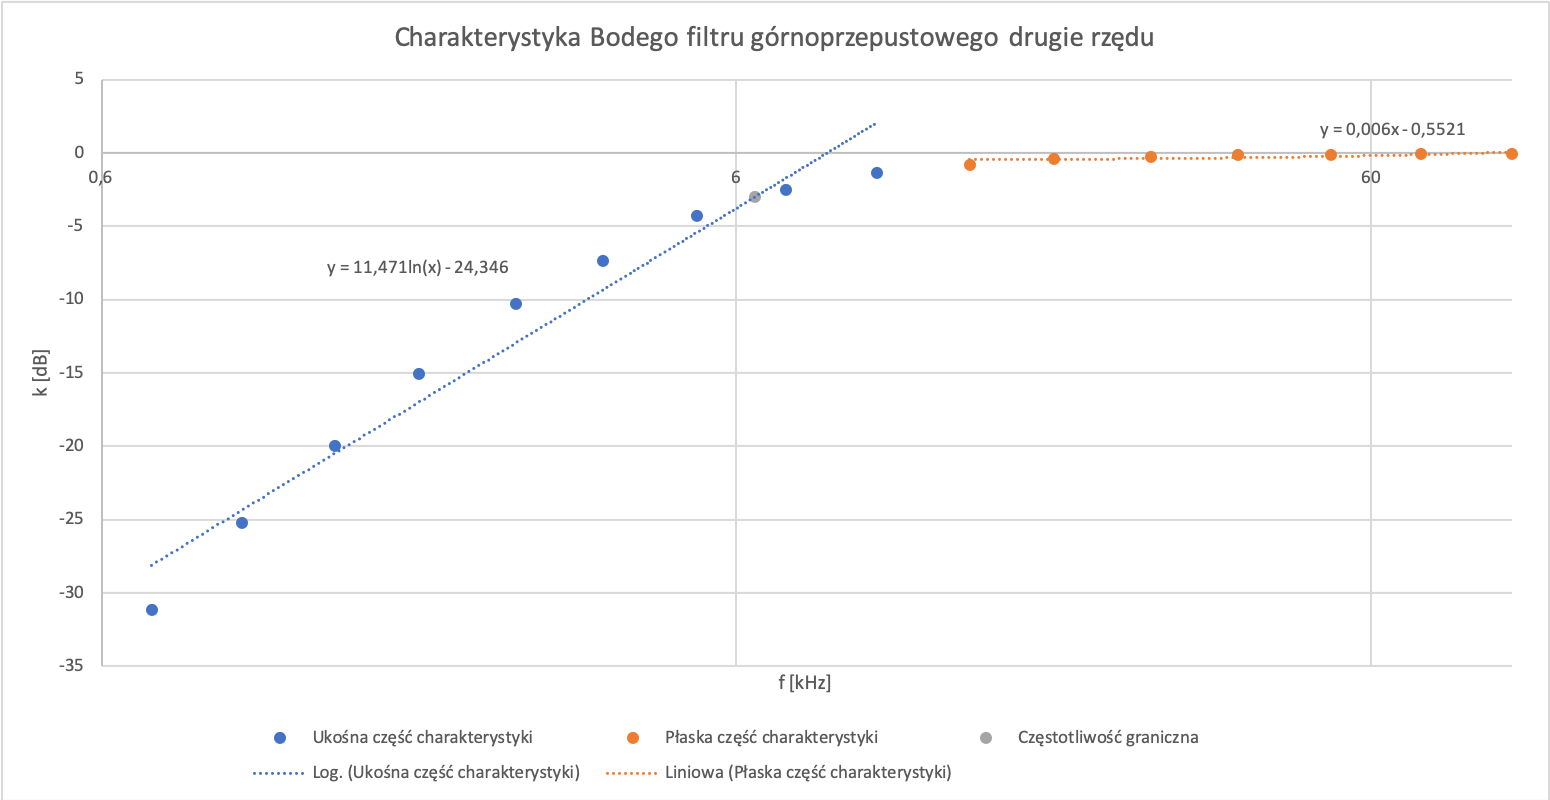
\includegraphics[width=15cm, height=9cm]{3_wykr}
\end{figure}

\paragraph{Zbadana częstotliwość graniczna $f_{g} = 6.42kHz$}

\paragraph{Częstotliwość graniczna została wyznaczona w identyczny sposób jak w filtrze górnoprzepustowym.}

\paragraph{Wartość współczynnika narastania ukośnej części charakterystyki $a = 11.471$}
\paragraph{Wartość współczynnika narastania płaskiej części charakterystyki $a = 0.0006$}

\paragraph{Jak widać powyżej współczynnik części płaskiej jest bardzo mały, a więc filtr przepuszcza dolne częstotliwości zgodnie z oczekiwaniami. }

\paragraph{Zbadane narastanie wyniosło $26.41 \frac{dB}{dek}$, również na wykresie możemy zaobserwować różnicę w narastaniu wynikającą z wykorzystania filtru II rzędu o różnych częstotliwościach granicznych. Dobierając odpowiedni opór na rezystorze możemy kontrolować }

\newpage

\begin{figure}[h]
\centering
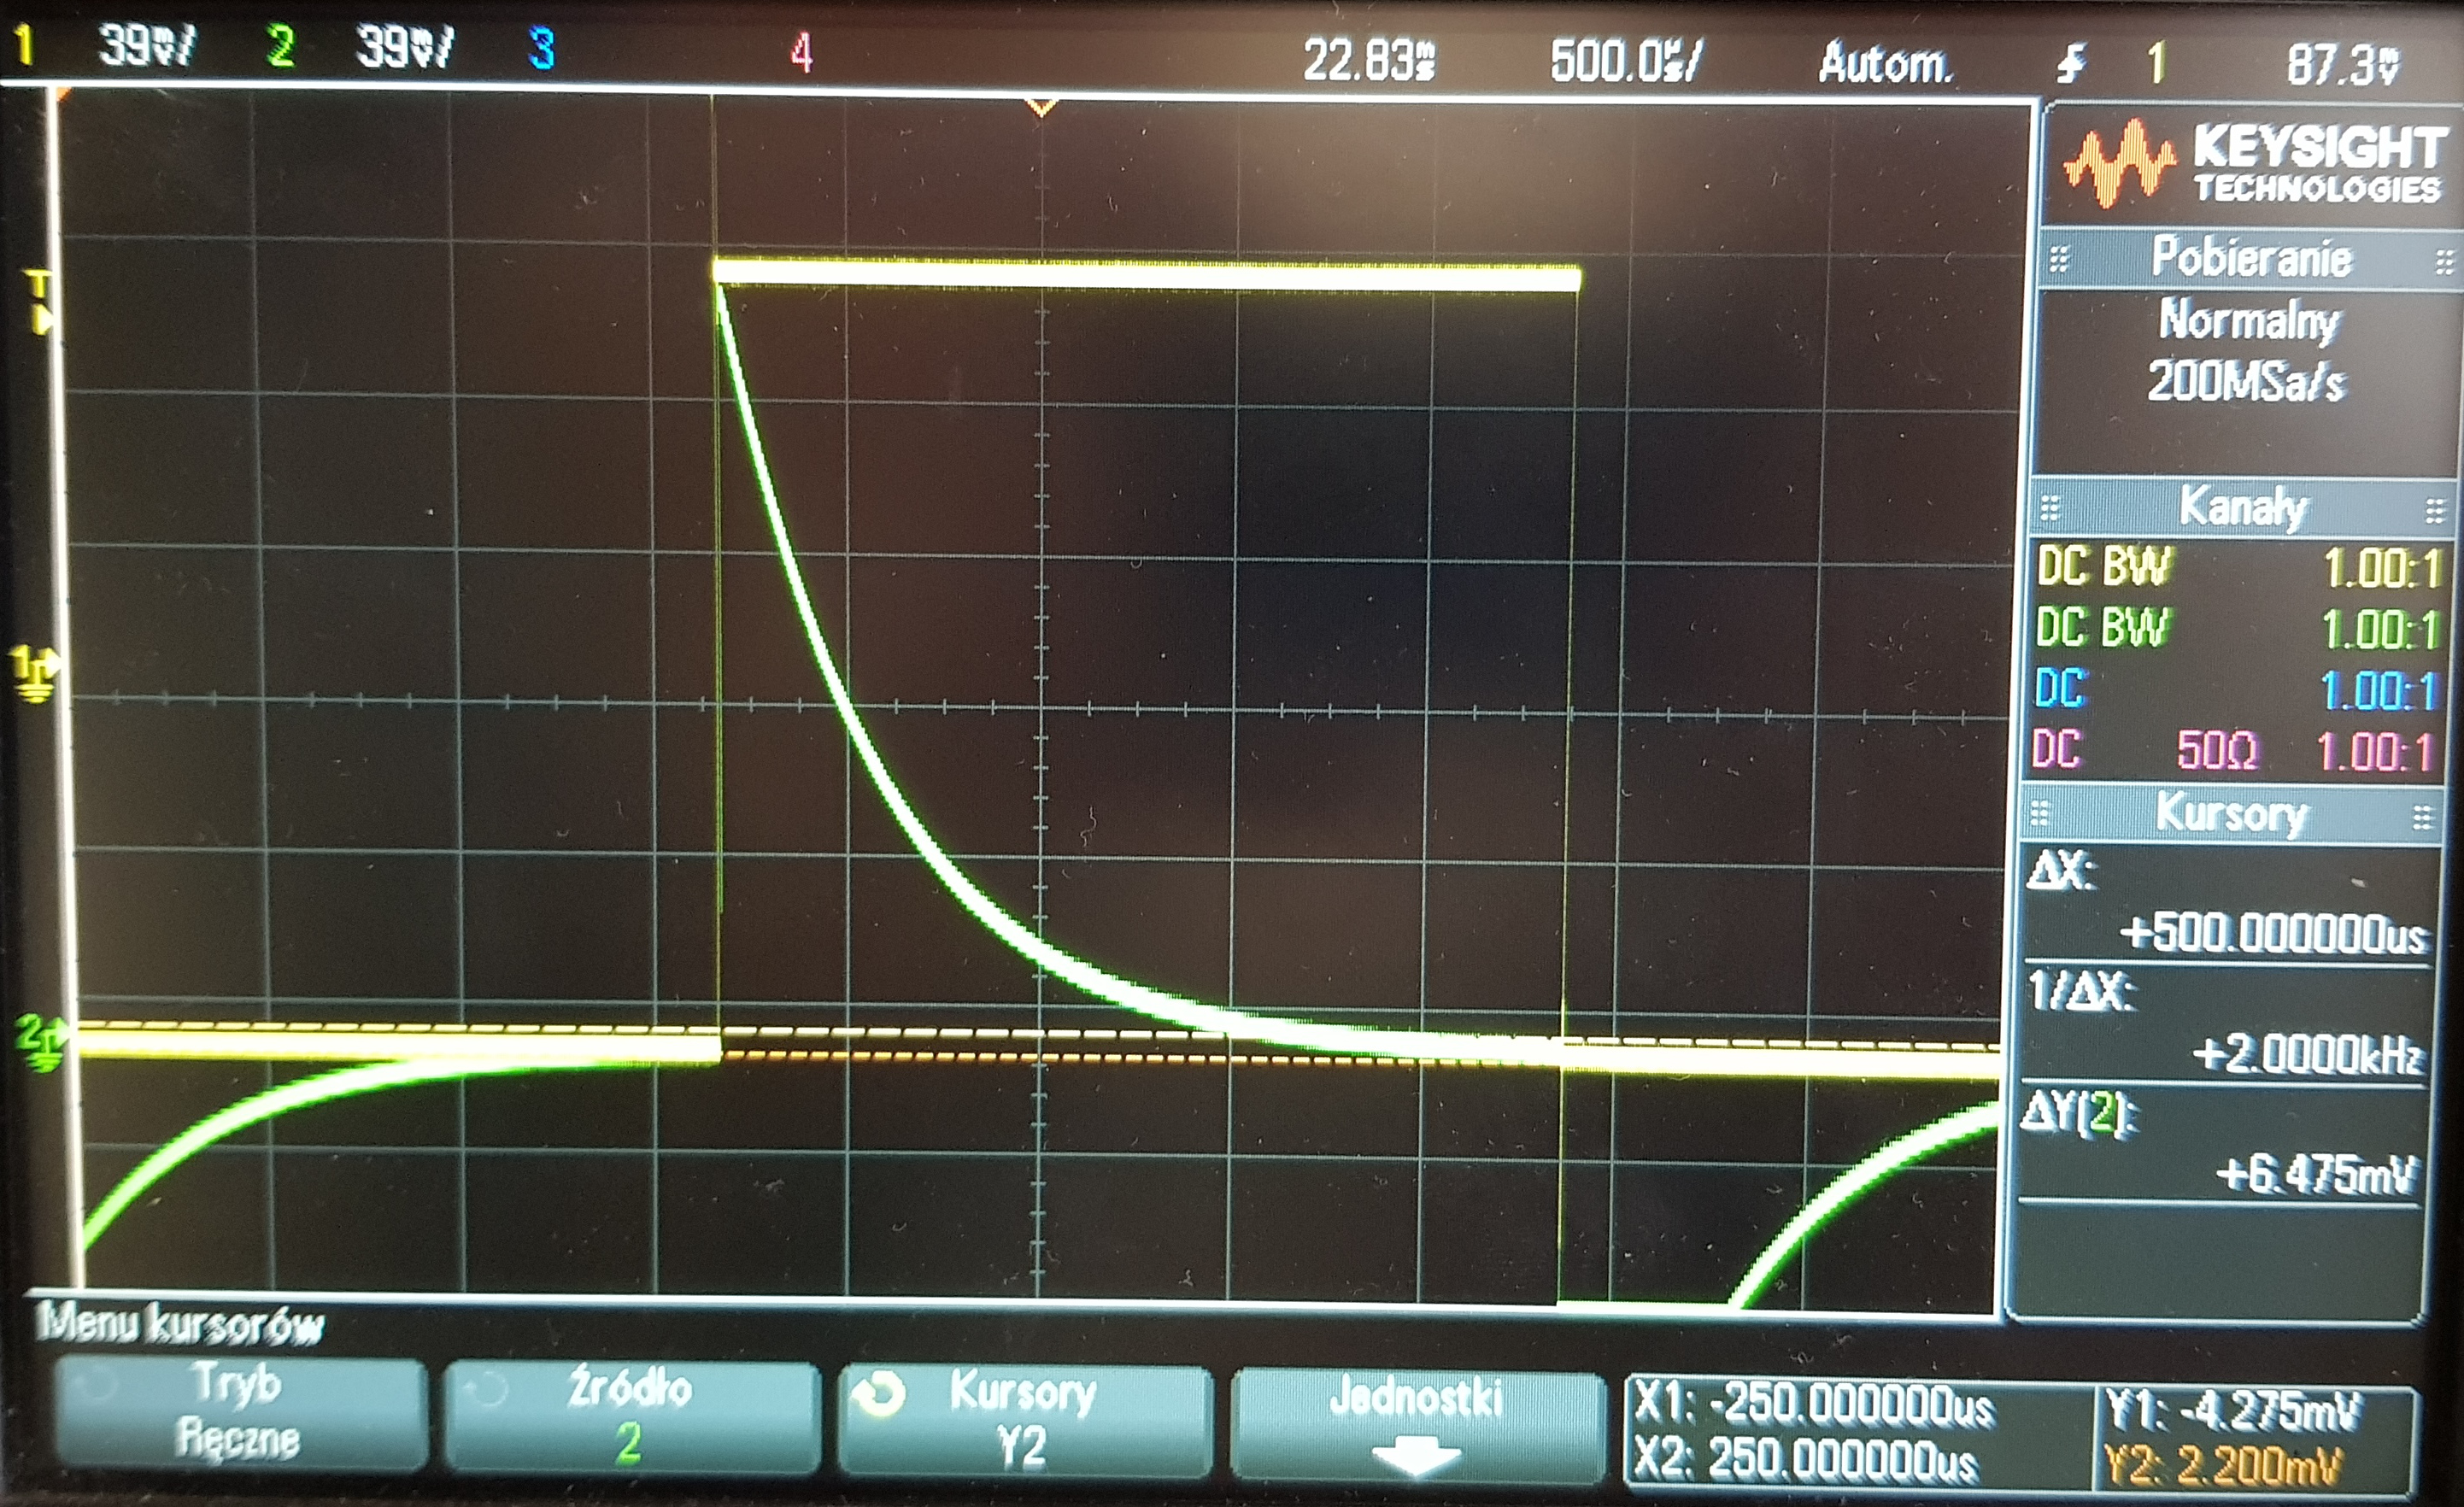
\includegraphics[width=15cm, height=9cm]{przerzut}
\end{figure}

\paragraph{Jak widać na powyższym obrazku widać przerzut, który jest spowodowany złym doborem oporu. Na kolejnym obrazku prezentujemy próbę niwelacji efektu.}

\paragraph{\\ \, \\}

\begin{figure}[h]
\centering
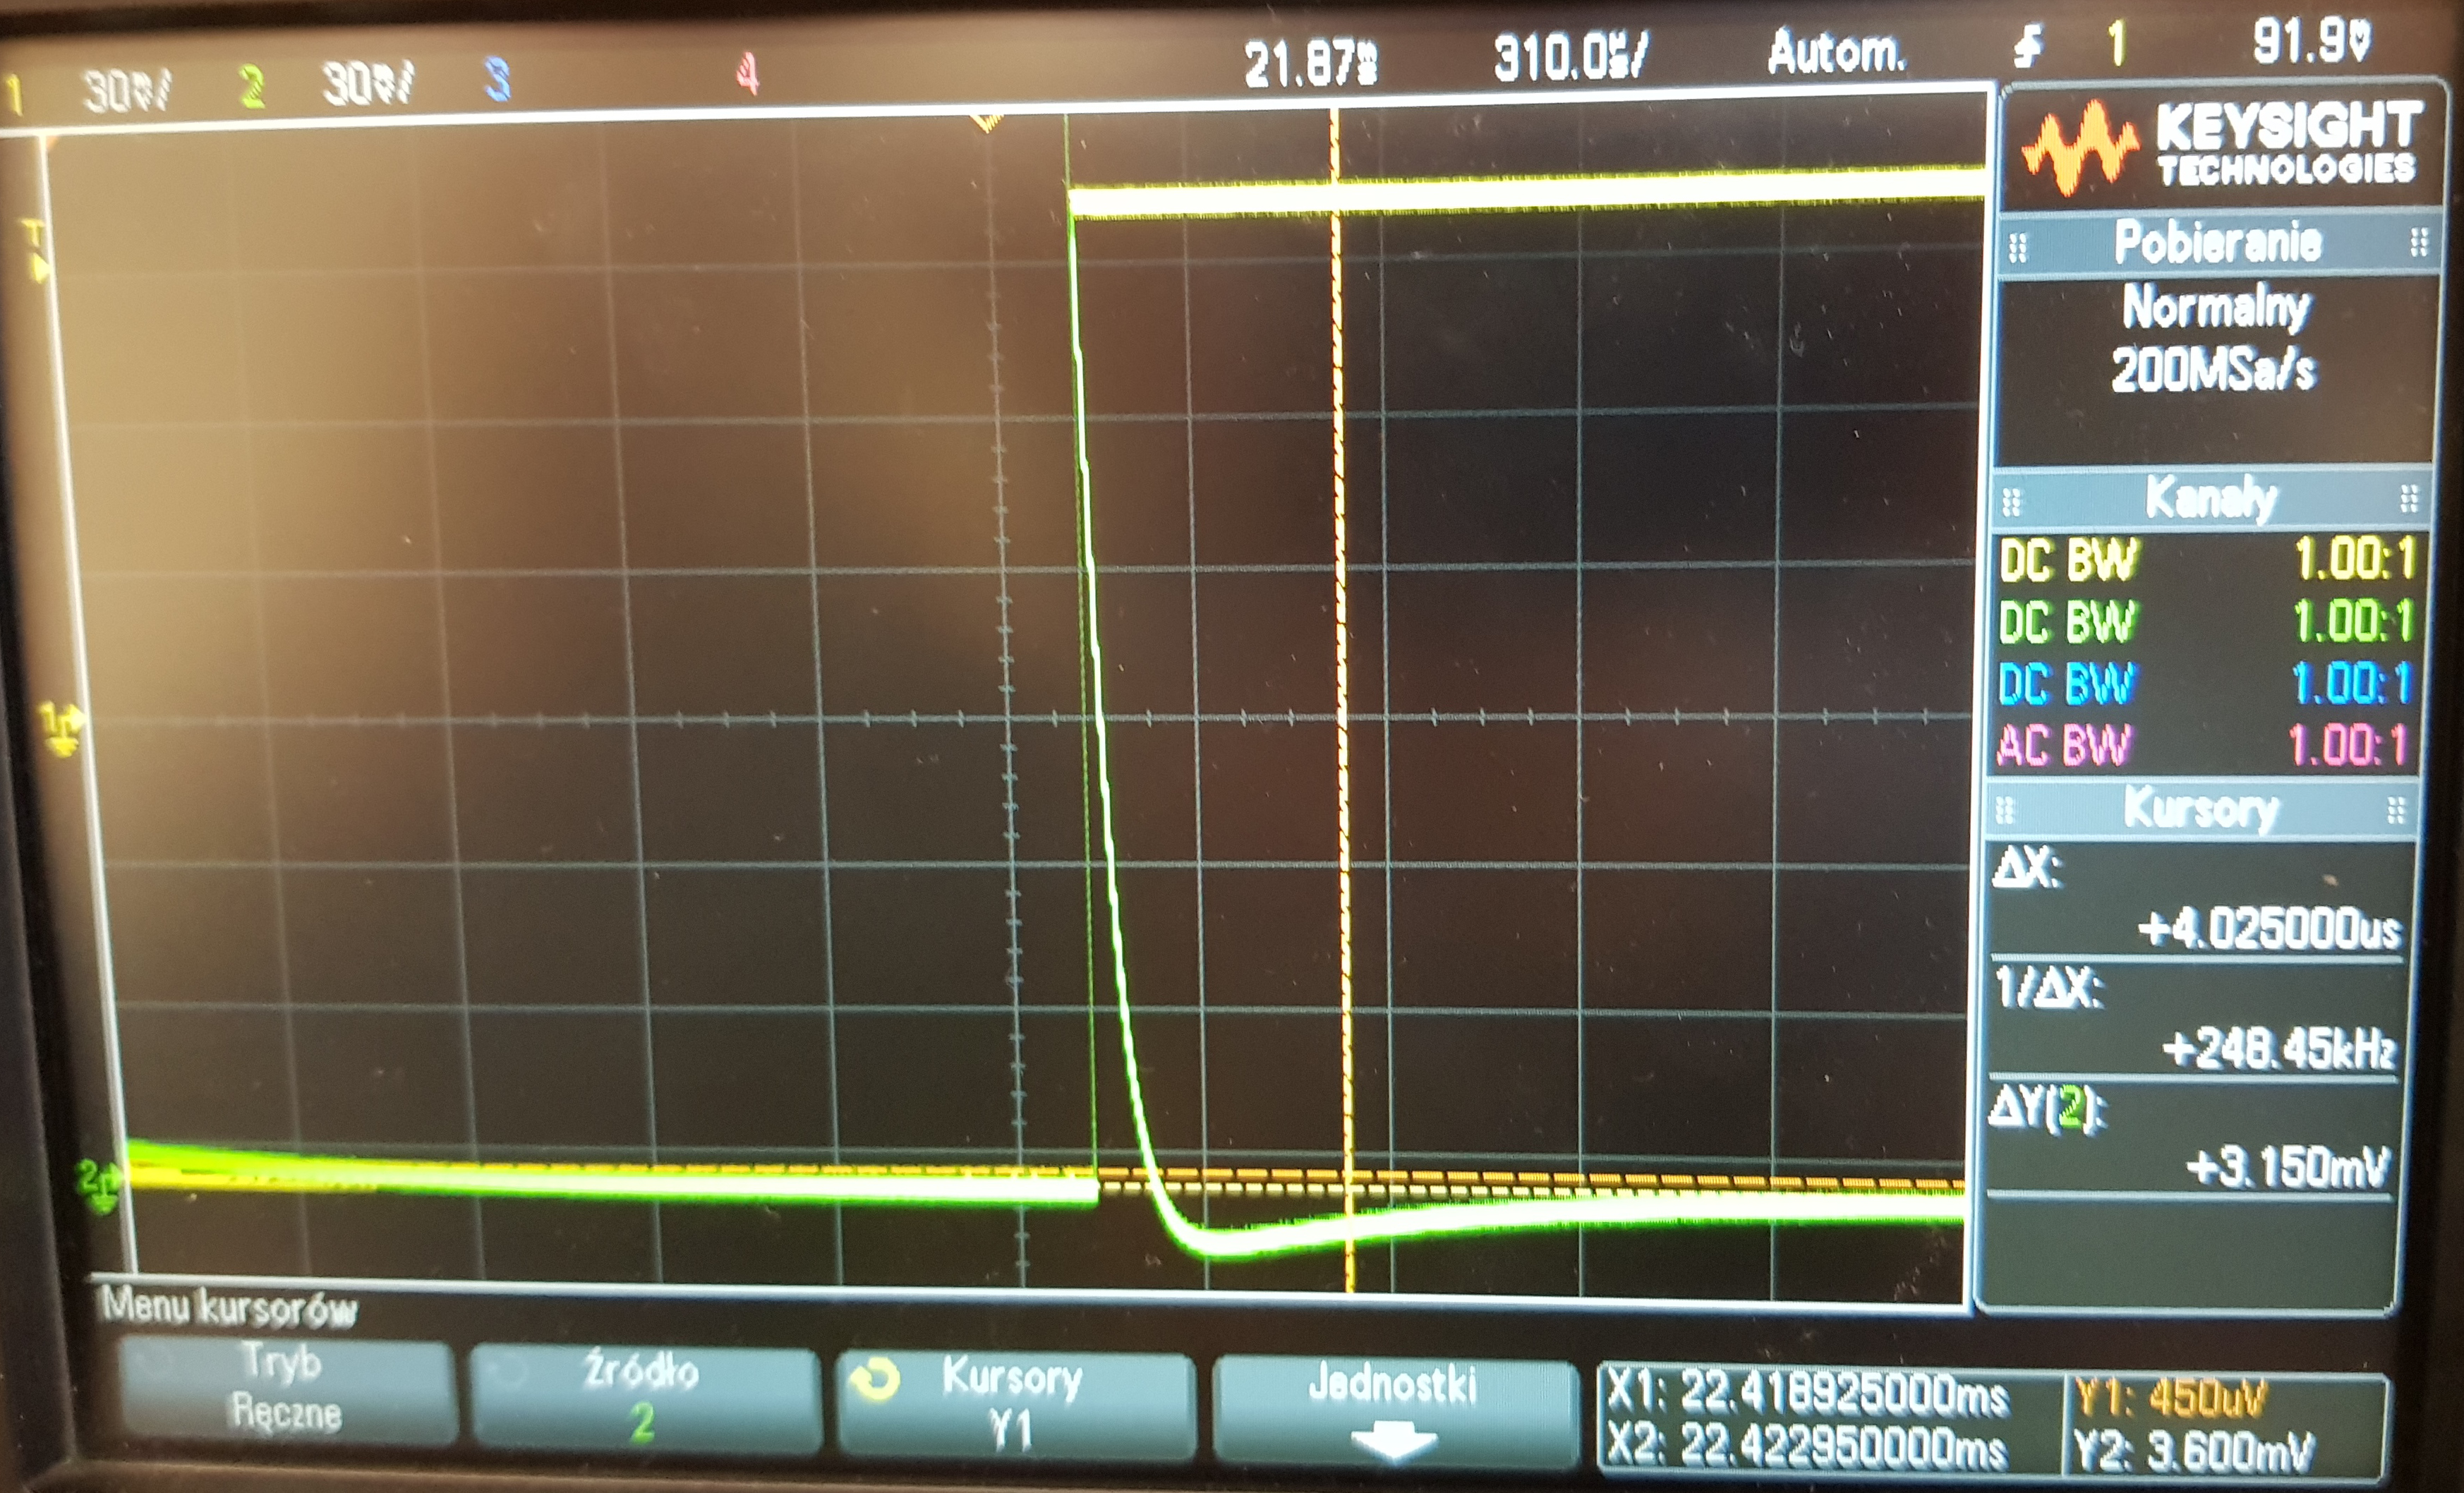
\includegraphics[width=15cm, height=9cm]{bez_przerzutu}
\end{figure}

\newpage

\subsection{Filtry aktywne}

\begin{figure}[h]
\centering
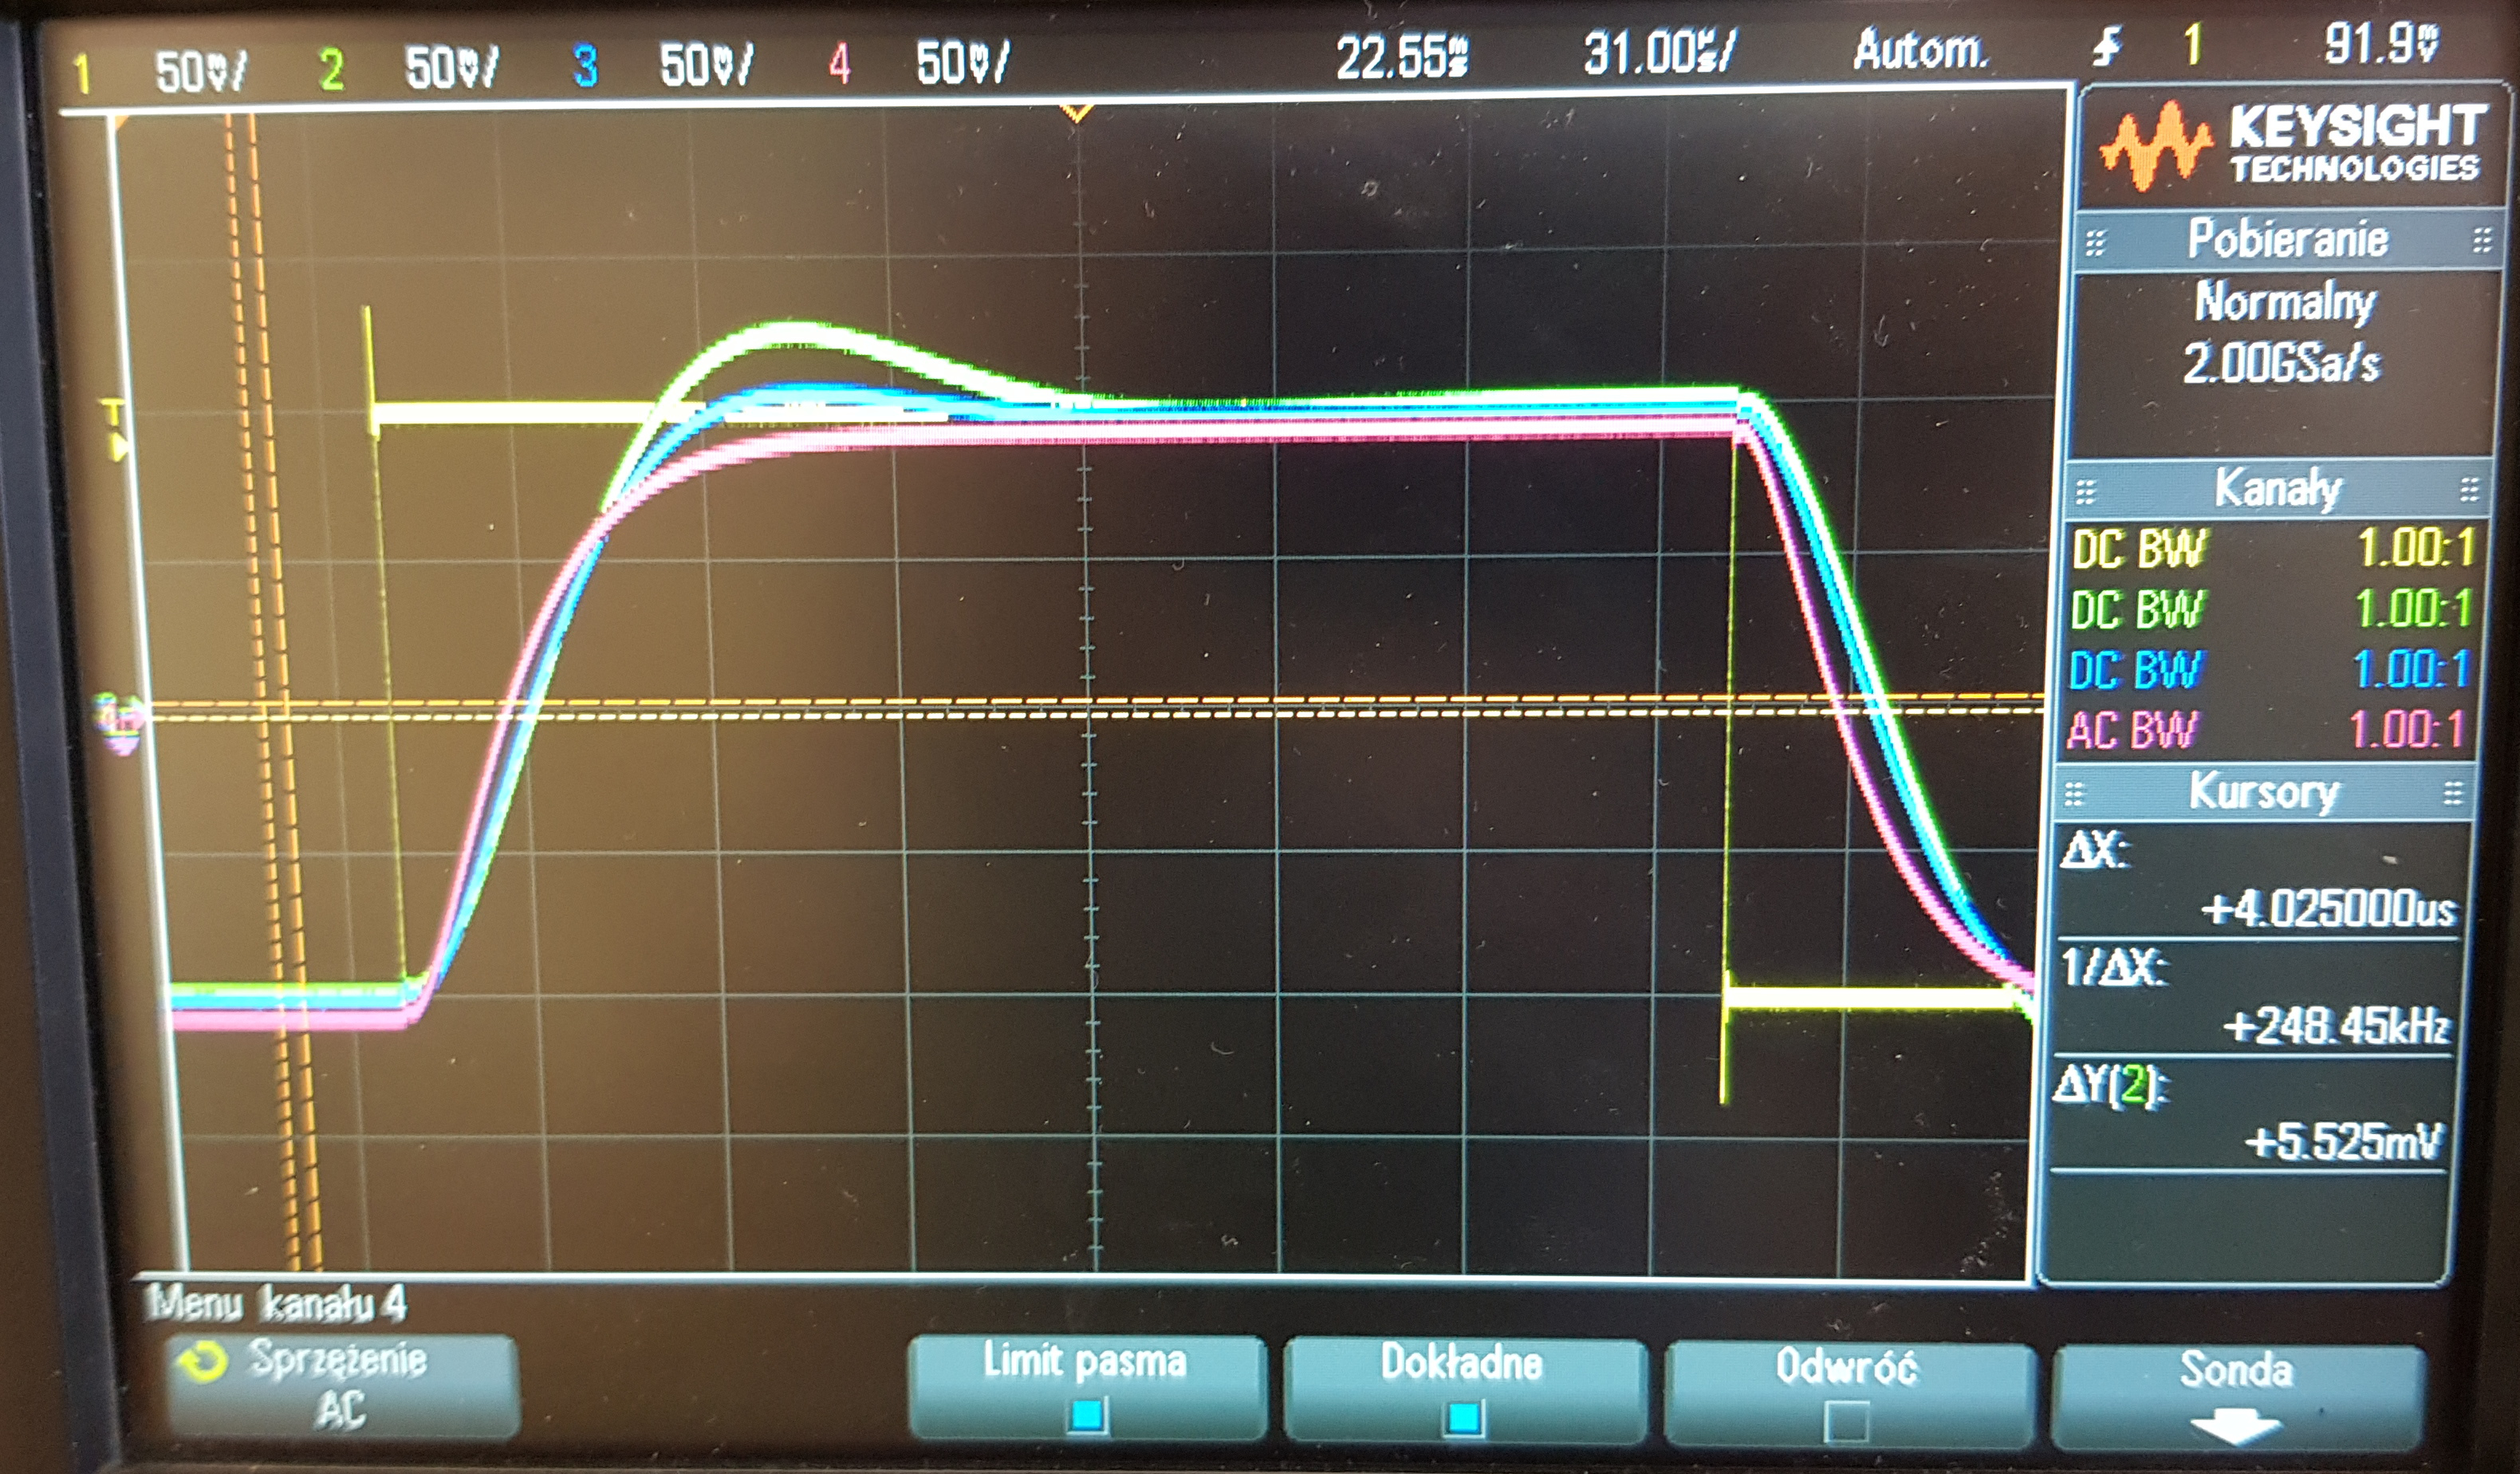
\includegraphics[width=15cm, height=9cm]{aktywne}
\end{figure}

\paragraph{Dla każdego z filtrów wyznaczyliśmy współczynnik wzmocnienia za pomocą przekształcenia wzoru na dobroć filtru oraz wykorzystaliśmy wyznaczone wartości dobroci dla poniższych filtrów.}

\subsubsection{Filtr Bessel'a}

\begin{figure}[h]
\centering
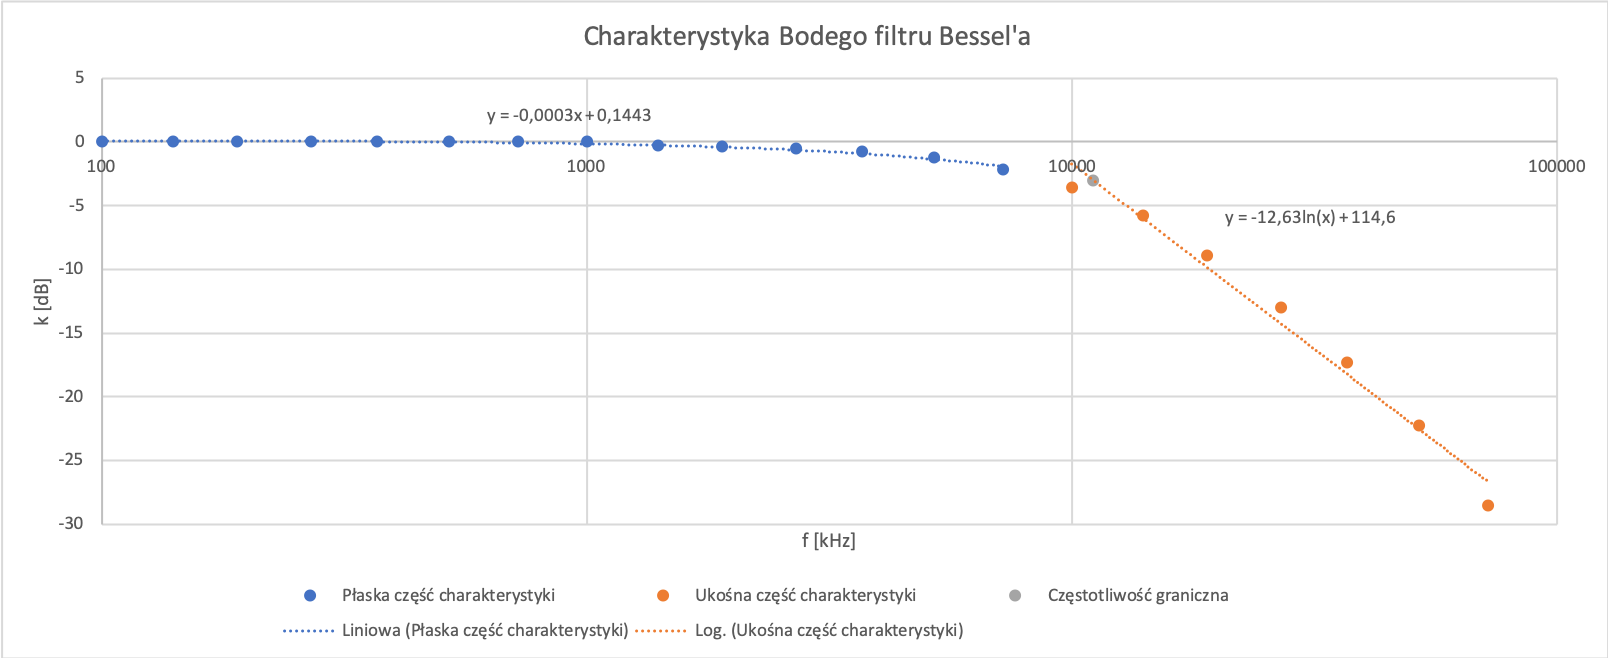
\includegraphics[width=15cm, height=9cm]{4_wykr_bessel}
\end{figure}

\paragraph{Zbadana częstotliwość graniczna $f_{g} = 11.06kHz$}

\paragraph{Wartość współczynnika narastania ukośnej części charakterystyki $a = -12.63$}
\paragraph{Wartość współczynnika narastania płaskiej części charakterystyki $a = 0.0003$}

\paragraph{Wyliczony współczynnik wzmocnienia: $k = 1$}

\paragraph{Zbadane opadanie wyniosło $-29.08 \frac{dB}{dek}$}

\subsubsection{Filtr Butterworth'a}

\begin{figure}[h]
\centering
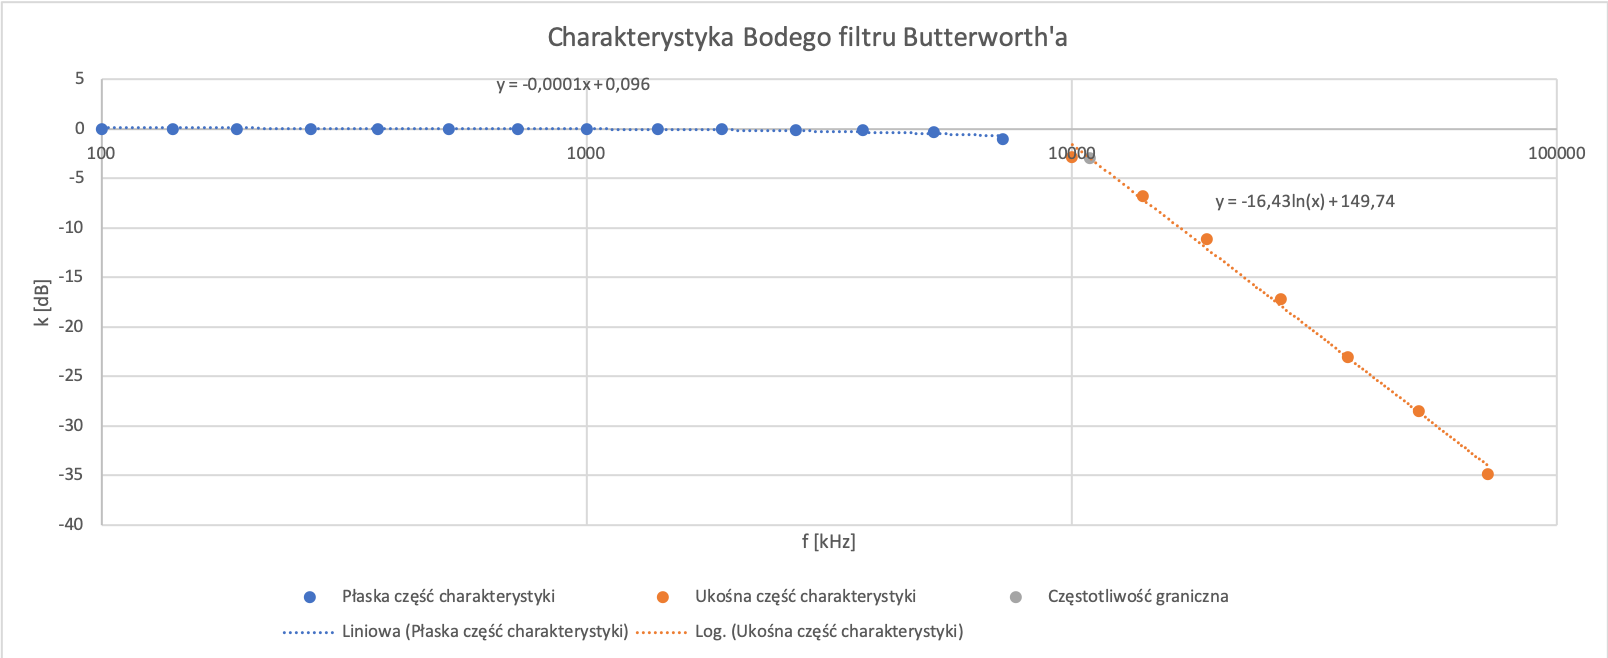
\includegraphics[width=15cm, height=9cm]{4_wykr_butterworth}
\end{figure}

\paragraph{Zbadana częstotliwość graniczna $f_{g} = 10.89kHz$}

\paragraph{Wartość współczynnika narastania ukośnej części charakterystyki $a = -16.43$}
\paragraph{Wartość współczynnika narastania płaskiej części charakterystyki $a = -0.0001$}

\paragraph{Wyliczony współczynnik wzmocnienia: $k = 2.99$}

\paragraph{Zbadane opadanie wyniosło $-37.83 \frac{dB}{dek}$}

\newpage

\subsubsection{Filtr Chebyshev'a}

\begin{figure}[h]
\centering
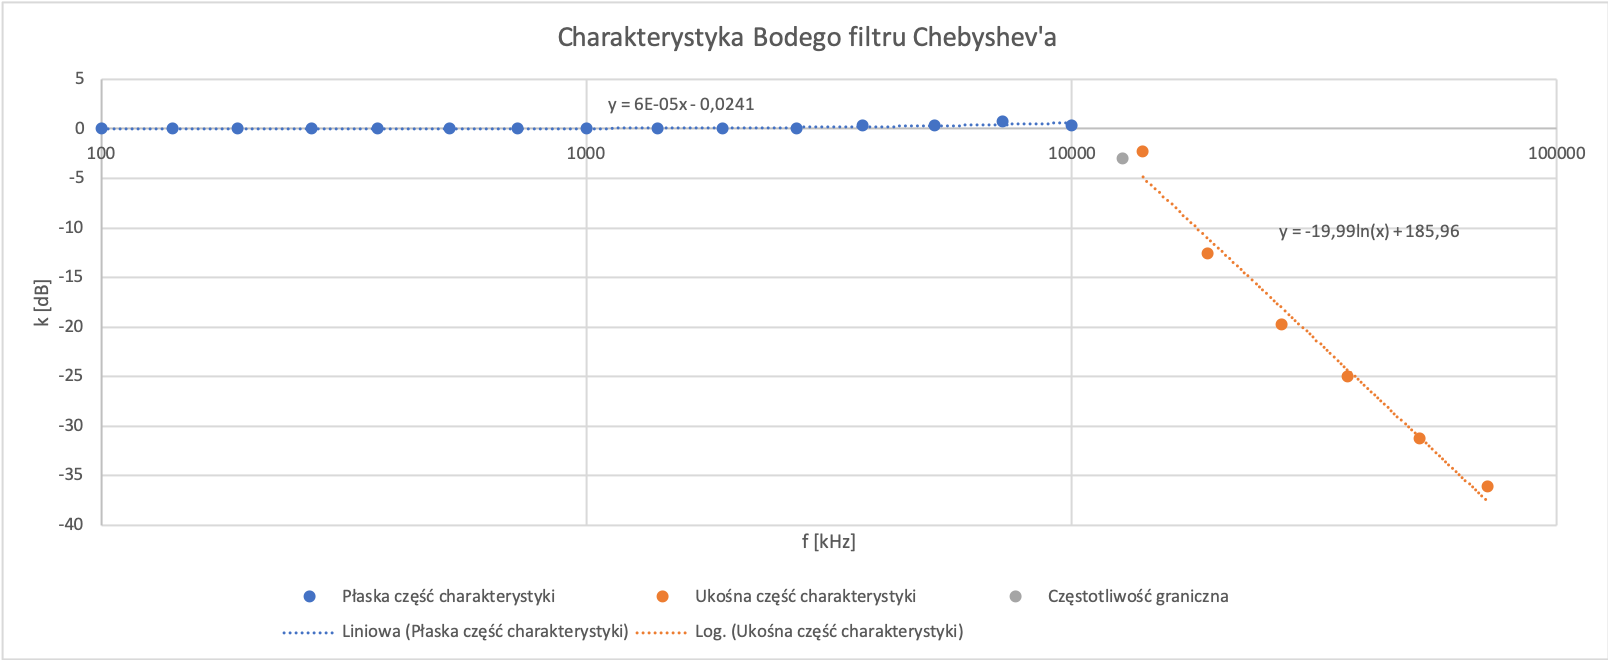
\includegraphics[width=15cm, height=9cm]{4_wykr_chebyshev}
\end{figure}

\paragraph{Zbadana częstotliwość graniczna $f_{g} = 12.74kHz$}

\paragraph{Wartość współczynnika narastania ukośnej części charakterystyki $a = -19.99$}
\paragraph{Wartość współczynnika narastania płaskiej części charakterystyki $a = 0.00006$}

\paragraph{Wyliczony współczynnik wzmocnienia: $k = 6.20$}

\paragraph{Zbadane opadanie wyniosło $-46.02 \frac{dB}{dek}$}

\paragraph{\,}

\end{justify}
\end{document}